\section{The compiler pipeline}

\todo{Assigned Jakob}

\begin{figure}[h!]
\centering
  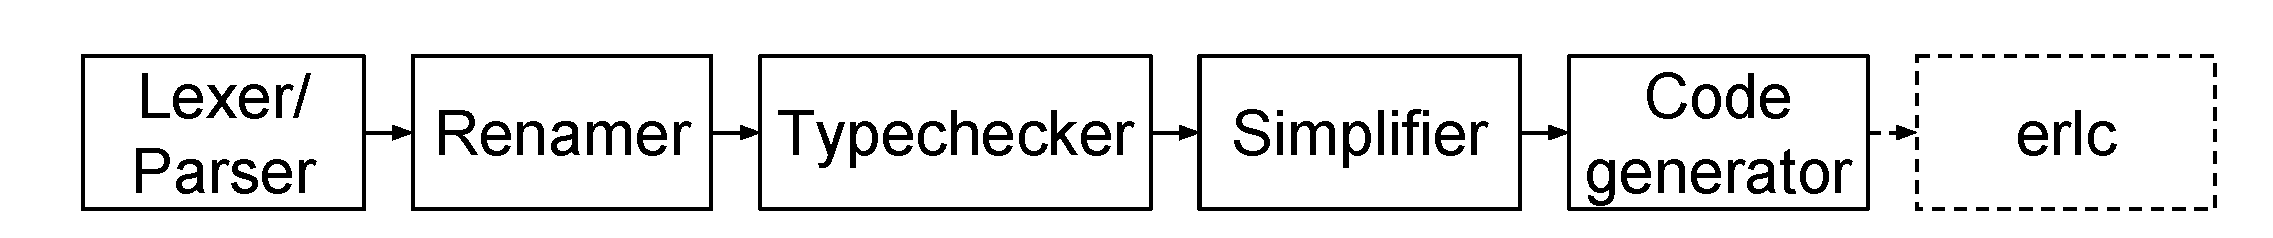
\includegraphics[width=0.6\pdfpagewidth]{figure/pipeline}
  \caption{Hopper's pipeline}
  \label{fig:pipeline}
\end{figure}

The core compiler functionality in Hopper is built to work on a single source file at a time. In order to support programs consisting of multiple modules the Hopper compiler, given a top-level module, is able to generate a compilation order for all modules in that program so that they can be compiled one at a time (see section~\ref{sec:dai_modules}).

As seen in figure~\ref{fig:pipeline}, the Hopper language has five major steps in its compiler pipeline before it hands over to the Erlang compiler. Each step works on the source code representation in a certain way.

The steps can be summarized as follows: the lexer and parser read in text files and convert them to an abstract representation, the renamer then simplifies this representation for the type checker. The type checker confirms and determines the types of all expressions. Lastly  there is another simplifying step before the code generator, which produces Core Erlang code. The Erlang compiler is then invoked on the produced Core Erlang code, and the result is Erlang assembly which can be run on the BEAM VM.